\section{Zadání}

Je dán anonymizovaný dataset o výsledcích léčby pacientů s mozkovou příhodou ve Fakultní nemocnici Plzeň za roky 2016 a 2017.
U pacientů je mimo jiné identifikován etiologický typ mozkové mrtvice, klinický výsledek (škála mRS), míra vstupního deficitu (škála NIHSS), přítomnost rizikových faktorů.
Data nejsou úplná, často jsou některé hodnoty neznámé.

\subsection{Úkoly}

\begin{enumerate}
    \item Zhodnoťte závislosti dobrého klinického výsledku (mRS-out: hodnota 1 oproti 0), případně mortalitu (mRS-1Y: hodnota 6 oproti 0-5) jednorozměrnou regresí na věku, pohlaví, vstupního NIHSS (TSS příjem) a rozdílu výstupní-vstupní NIHSS.
    \item Vytvořte Kaplan–Meierovy křivky přežití pro jednotlivé stanovené diagnózy a podrobně popište proces vytvoření a její vlastnosti.
\end{enumerate}

\section{Zhodnocení závislostí}

Abychom mohli objektivně zhodnotit závislosti přítomné v datech je nutné znát data samotná.
Podívejme se nejdříve na histogramy ukazující počty pacientů vůči jejich věku, diagnózám a hodnotě mRS po jednom roce.

\begin{figure}[htbp]
    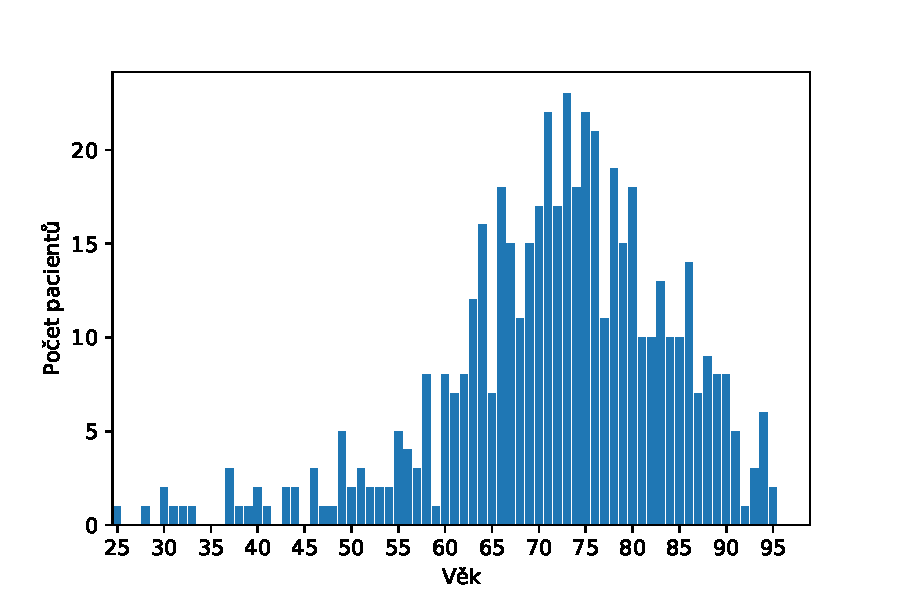
\includegraphics[width=.6\textwidth]{img/image_0.pdf}
    \centering
    \caption{Histogram počtu pacientů v závislosti na věku}
    \label{img:age-histogram}
\end{figure}
\FloatBarrier

Z histogramu~\ref{img:age-histogram} vyplývá, že většina pacientů ve studii je starší 60 let.
Data odpovídají trendu výskytu ischemických příhod, které se v populaci vyskytují výrazně více právě od této věkové hranice.

\begin{figure}[htbp]
    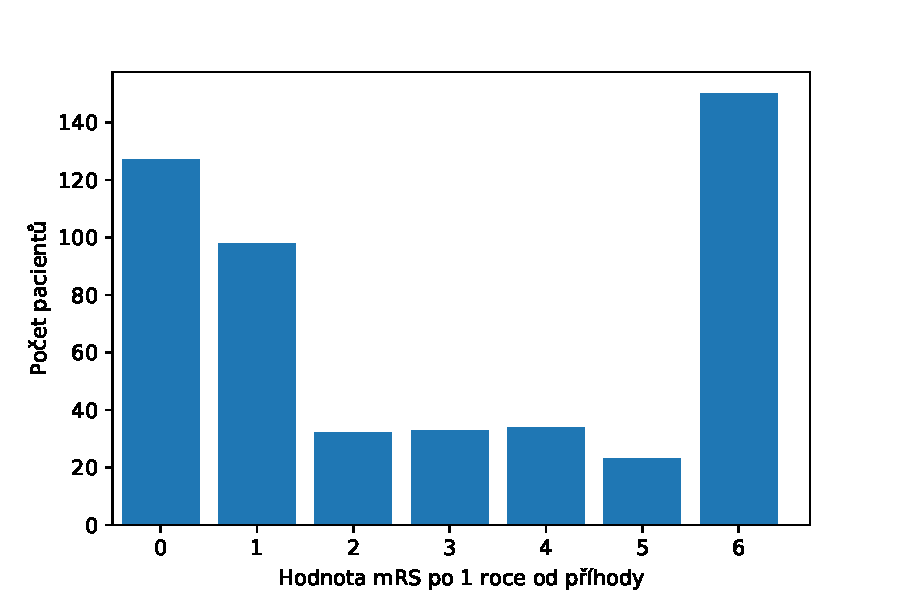
\includegraphics[width=.6\textwidth]{img/image_1.pdf}
    \centering
    \caption{Histogram počtu pacientů v závislosti na hodnotě mRS po jenom roce}
    \label{img:mrs-histogram}
\end{figure}
\FloatBarrier

Histogram číslo~\ref{img:mrs-histogram} napovídá, největší procento z celkového počtu pacientů se nedožilo jednoho roku od ischemické příhody.
Na druhou stranu, vysoké procento pacientů žilo a to dokonce s žádnými následky (hodnota 1 na histogramu) či bez zřetelného omezení, schopno vykonávat běžné denní aktivity (hodnota 2).

\begin{figure}[htbp]
    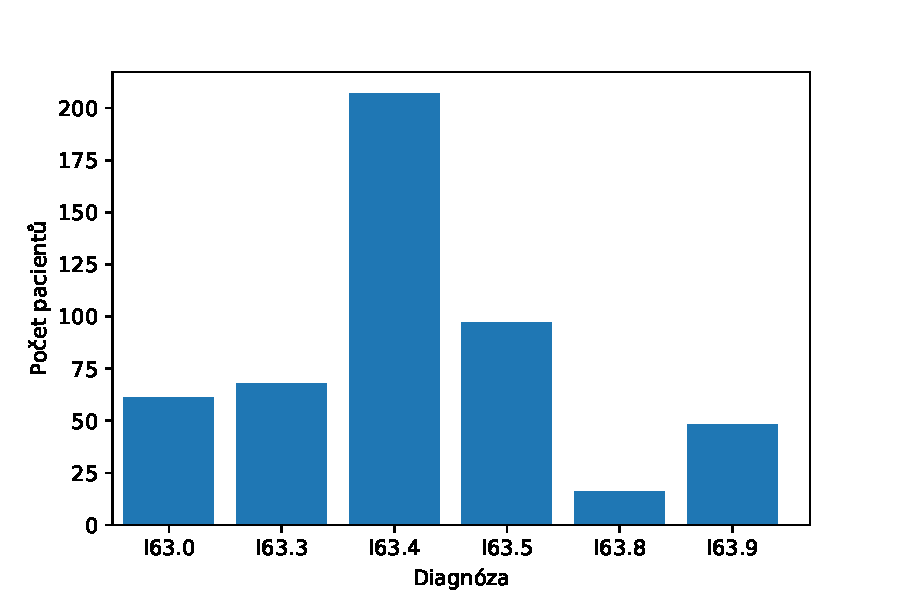
\includegraphics[width=.6\textwidth]{img/image_2.pdf}
    \centering
    \caption{Histogram počtu pacientů v závislosti na diagnóze}
\end{figure}
\FloatBarrier

Třetí histogram ukazuje, že v nasbíraných datech se nejvíce vyskytují pacienti s diagnózou číslo 4.
Nedostatek dat o jiných diagnózách zcela jistě ovlivní výsledky z Kaplan–Meierovy analýzy a pravděpodobně by tedy nebylo žádoucí vyvozovat z výsledných křivek statisticky relevantní závěry.

Pro vysvětlení grafu uvádím seznam diagnóz s jejich očíslováním:

\begin{itemize}
    \item I63.0: Cerebral infarct, large vessel disease with significant carotid stenosis,
    \item I63.3: Cerebral infarct, other large vessel disease,
    \item I63.4: Cerebral infarct, cardic emboli,
    \item I63.5: Cerebral infarct, small vessel / lacunar,
    \item I63.8: Cerebral infarct, other / unusual cause,
    \item I63.9: Cerebral infarct, multiple / unknown cause.
\end{itemize}

Pro zobrazení závislostí v první úloze byl zvolen logisticko-regresní model (bohužel kvůli zvolenému způsobu řešení není možné získat parametry dané křivky).

\begin{figure}[htbp]
    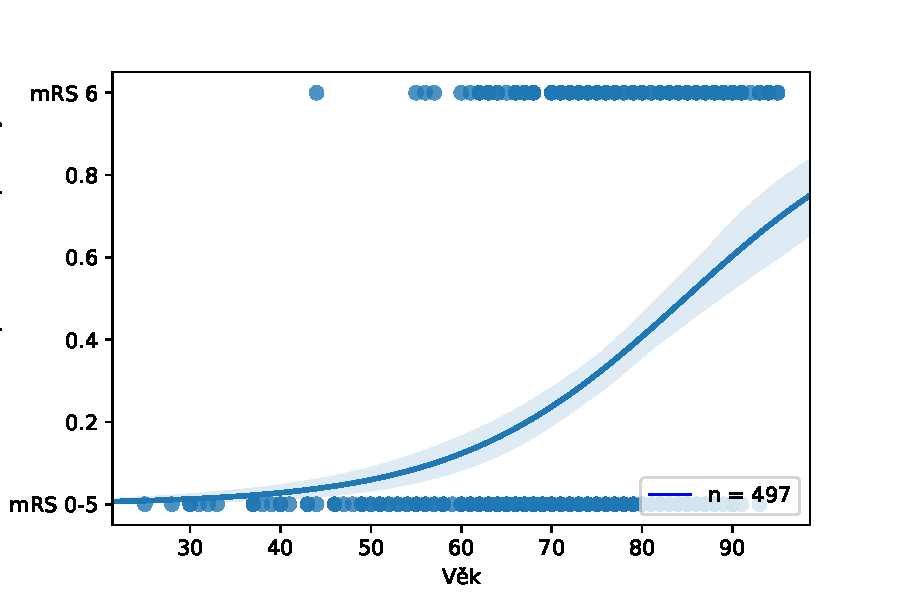
\includegraphics[width=.6\textwidth]{img/image_3.pdf}
    \centering
    \caption{Závislost mortality na věku}
    \label{img:mrs-age}
\end{figure}
\FloatBarrier

Na grafu~\ref{img:mrs-age} pozorujeme, že čím je pacient starší, tím větší je riziko, že do roka po příhodě umře.
Tato závislost je přirozená a zcela intuitivní, nehledě na data, která máme spíše pro pacienty pokročilejšího věku.

\begin{figure}[htbp]
    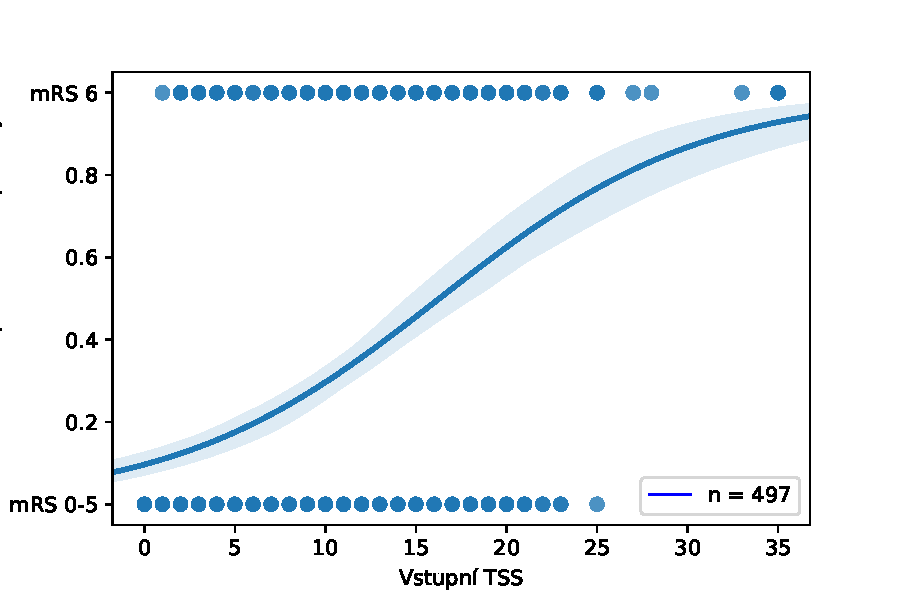
\includegraphics[width=.6\textwidth]{img/image_4.pdf}
    \centering
    \caption{Závislost mortality na celkovém NIHSS skóre}
    \label{img:mrs-tss}
\end{figure}
\FloatBarrier

\begin{figure}[htbp]
    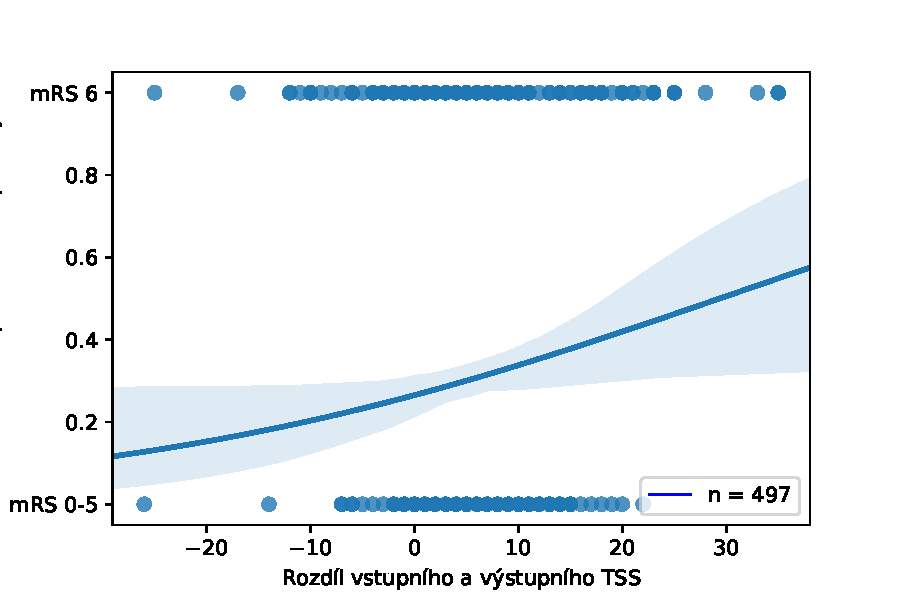
\includegraphics[width=.6\textwidth]{img/image_5.pdf}
    \centering
    \caption{Závislost mortality na rozdílu vstupního a výstupního NIHSS skóre, kladné číslo znamená zlepšení stavu (nižší výstupní hodnota), záporné číslo znamená zhoršení}
    \label{img:mrs-tss2}
\end{figure}
\FloatBarrier

Grafy~\ref{img:mrs-tss} a~\ref{img:mrs-tss2} jsou též velice intuitivní.
Pacienti s lepším hodnocením dle škály NIHSS mají obecně větší naději na přežití.
Zajímavý je graf~\ref{img:mrs-tss2}, který tvoří téměř lineární závilost, ačkoliv vykreslená je logistická funkce.

Poslední závislost - mortality na pohlaví pacienta - zobrazme kontingenční tabulkou.

\begin{table}[htbp]
    \centering

    \begin{tabular}{ccc}
        \toprule
        Died    & False & True  \\
        Sex     &       &       \\
        \midrule
        Female  & 153   & 73    \\
        Male    & 194   & 77    \\
        \bottomrule
    \end{tabular}    
    
    \caption{Mortalita v závislosti na pohlaví}
    \label{table:sex-mortality}
\end{table}
\FloatBarrier

\newpage
\section{Analýza přežití}

Analýza přežití, známá v angličtině pod pojmem \enquote{survival analysis} je odvětvím statistiky, které se zabývá analýzou trvání procesu či života objektu až do okamžiku vzniku události zájmu, tzv. \enquote{time-to-event data}.
Toto odvětví má širokou škálu využití, od odhadování střední doby života, přes socio-ekonomické aplikace až po spolehlivostní inženýrství (\enquote{reliability theory}).

Pro analýzu je nutné sbírat data o událostech zájmu a zaznamenávat uplynulý čas od začátku sledování po vyskytnutí události.
V případě datasetu, dostupného k úloze, se jedná o pacienty u kterých je počáteční událostí projev ischemie mozku, tedy jeden z typů mrtvice.
Touto událostí pacient vstupuje do studie.
Za koncovou (sledovanou) událost považujme úmrtí pacienta na následky proběhlé mrtvice - tím může být mrtvice samotná či jiná doprovodná událost.

Při sledování dostupných dat narazíme na několik možných variant.
Buď data o koncové události pacienta máme k dispozici, nebo nemáme.
Taková data nazývají jako \enquote{cenzorovaná}.
Ať už jde o možnost, že nějaká událost nastala, ale netýkala se přímo oblasti zájmu (pacient umřel, ale ne na následky ischemie), případně nemohl být dále sledován pro účely studie (byl přeložen na jiné oddělení, či propuštěn z~nemocnice), nebo byla studie ukončena.

Nasbíraná data se dají transormovat do podoby \textit{funkce přežití}, \enquote{survival function}, vyjadřující pravděpodobnost, že pacient přežije po stanovenou dobu.
Jedna z takových funkcí je tzv. \enquote{follow-up method}.
Ta vyjadřuje za pomocí ekvidistantních časových úseků pravděpodobnost přežití do konce intervalu.

Další funkcí, která se běžně používá je Kaplan-Meierova.
Tato metoda byla roku 1958 vymyšlena Edwardem L. Kaplanem a Paulem Meierem.
Na rozdíl od první metody je pravděpodobnost přežití přepočítávána po každé nastalé události.

\subsection{Kaplan-Meier}

Pro výpočet Kaplan–Meierovy křivky potřebujeme data ve formě výskytů událostí v časových okamžicích.
Taková data dostaneme rozdílem datumů zařazení do studie a datumů úmrtí pacientů na následky sledované příhody.
Pacienti kteří nemají uveden datum úmrtí jsou \enquote{cenzorovaní}.
Při vykreslování jsem nerozlišoval zda pacient umřel na následky ischemie, nebo nikoliv.
Ve většině případů umřel právě na následky ischemie.
Opačných případů bylo pouze několik, v rámci zachování dostatečného vzorku dat je tedy začleňuji mezi skupinu která na ischemii umřela.
Příčinu skonu pacienta se z dat dovídáme pomocí poznámky v závorce za datem úmrtí.

\begin{figure}[htbp]
    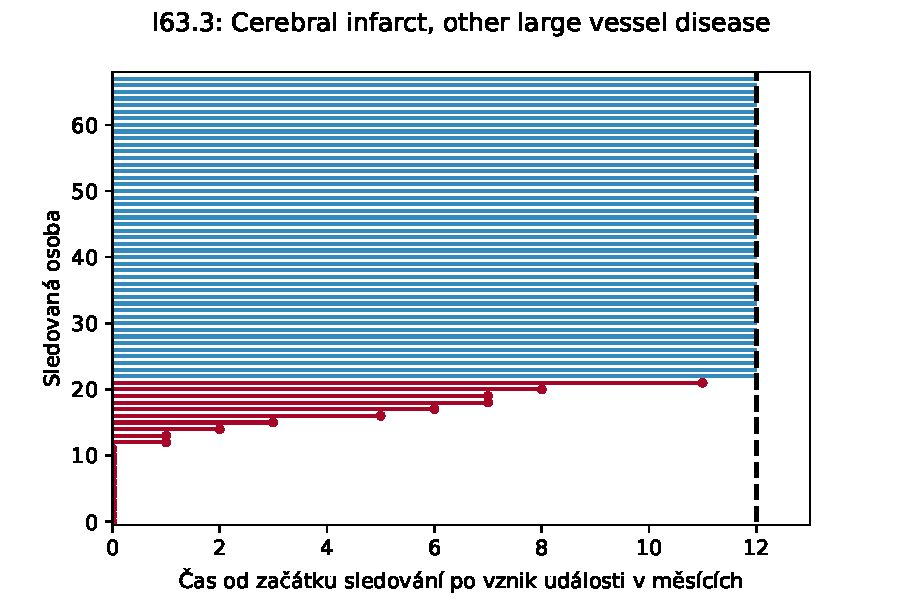
\includegraphics[width=.6\textwidth]{img/image_6.pdf}
    \centering
    \caption{Délky života pacientů od výskytu příhody do úmrtí (červená) nebo do konce studie (modrá) v měsících pro jednu diagnózu}
    \label{img:lifelines}
\end{figure}
\FloatBarrier

Po zobrazení zaznamenaných délek života od výskytu příhody do úmrtí nebo do konce studie dostaneme graf na obrázku~\ref{img:mrs-tss}.
Koncové časy událostí nám poslouží k výpočtů Kaplan–Meierovy křivky.

\subsection{Příklad výpočtu Kaplan-Meierovy křivky}

Výpočet funkce přežití ukáži na ilustračním příkladu.
Mějme sadu událostí v časech 2, 6, 6, 7, 15, 15, 16, 27, 30, 32.
Dále máme dvě cenzorované události a to v časech 2 a 10.

Vše vypíšeme do tabulky~\ref{table:kaplan-meier}.
Veškeré časy zapíšeme do sloupce \textit{Time}, počty sledovaných událostí v časech zapíšeme do sloupce \textit{Event}, počty cenzorovaných událostí do sloupce \textit{Censored}.
Sloupec \textit{Risk set} se snižuje podle počtu událostí, které nastaly.
Jeho počáteční hodnota je množství všech událostí.
Sloupec \textit{Factor} spočítáme podle uvedeného vzorce.
Je-li v čase 15 zbývající velikost množiny 6 a nastaly 2 události, pak vypočteme hodnotu ve sloupci jako \( 1 - \frac{2}{6} \) což jsou \( \frac{2}{3} \simeq 0.667 \).

Jako poslední zbývá spočítat hodnoty funkce přežití.
Tu dostaneme tak, že přenásobíme hodnotu ve sloupci \textit{Factor} s hodnotou funkce v předchozím časovém okamžiku.
Vezměme si tedy vypočítaný sloupec \textit{Factor} v čase 15, což odpovídá číslu \( 0.667 \).
Poslední událost nastala v čase 10 a hodnota sloupce \textit{Survival} je v tomto čase \( 0.642 \).
Tyto dvě hodnoty pronásobíme \( 0.642 \times 0.667 \) a dostáváme \( 0.428 \).
Hodnota v čase 0 musí být jedna - žádná událost do té doby nenastala, pravděpodobnost přežití musí být tedy rovna jedné.
V případě, že se nalázají události i v čase 0, pak zavádíme čas \( -1 \), ve kterém je hodnota pravděpodobnosti přežití rovna jedné.

\begin{table}[htbp]
    \centering

    \begin{tabular}{SccSSS}  
        \toprule
        Time    & Event & Censored  & Risk set  & Factor    & Survival  \\
        t       & d     & c         & n         & \factor   & \survival \\
        \midrule
         0      &       &           & 12        &           & 1         \\
         2      & 1     & 0         & 12        & 0.917     & 0.917     \\
         3      & 0     & 1         & 11        & 1         & 0.917     \\
         6      & 2     & 0         & 10        & 0.8       & 0.734     \\
         7      & 1     & 0         &  8        & 0.875     & 0.642     \\
        10      & 0     & 1         &  7        & 1         & 0.642     \\
        15      & 2     & 0         &  6        & 0.667     & 0.428     \\
        16      & 1     & 0         &  4        & 0.75      & 0.321     \\
        27      & 1     & 0         &  3        & 0.667     & 0.214     \\
        30      & 1     & 0         &  2        & 0.5       & 0.107     \\
        32      & 1     & 0         &  1        & 0         & 0         \\
        \bottomrule
    \end{tabular}    
    
    \caption{Kaplan–Meierova tabulka}
    \label{table:kaplan-meier}
\end{table}
\FloatBarrier

\subsection{Výsledky}

Po aplikaci výpočtu na dostupná data dostáváme výsledky na grafu.
Je vidět, že pro výpočet křivek pro některé diagnózy nebylo dostatek dat.
Výsledky jsou tedy v těchto případech pouze ilustrační.

Světle modrá zóna kolem křivek jsou intervaly spolehlivosti.
Ten je v tomto případě počítám pomocí Greenwoodovy metody, kde \( z_{\alpha} \) je kvantil alfa normálního rozdělení se střední hodnotou rovnou hodnotě funkce přežití a vypočtenou variancí.

\[ \hat{S}(t) \pm z_{\alpha / 2} \sqrt{\survivalvar} \]
\[ \survivalvar = \hat{S}(t)^{2} \sum_{t_{i} \leq t} \frac{d_{i}}{n_{i}\left(n_{i}-d_{i}\right)} \]

\begin{figure}[htbp]
    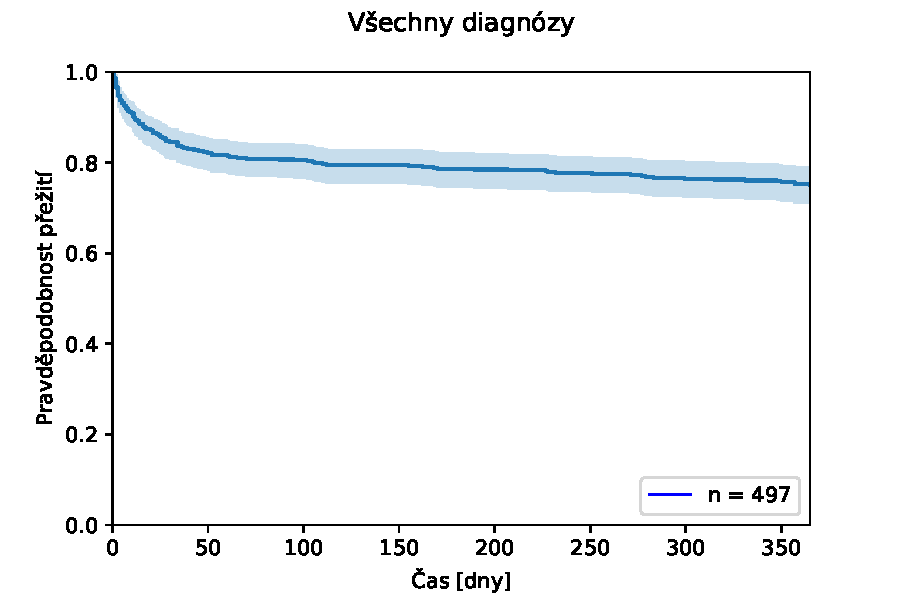
\includegraphics[width=.8\textwidth]{img/image_7.pdf}
    \centering
    \caption{Souhrnná Kaplan–Meierova křivka přežití}
\end{figure}
\FloatBarrier

\begin{figure}[htbp]
    \begin{tabular}{cc}

        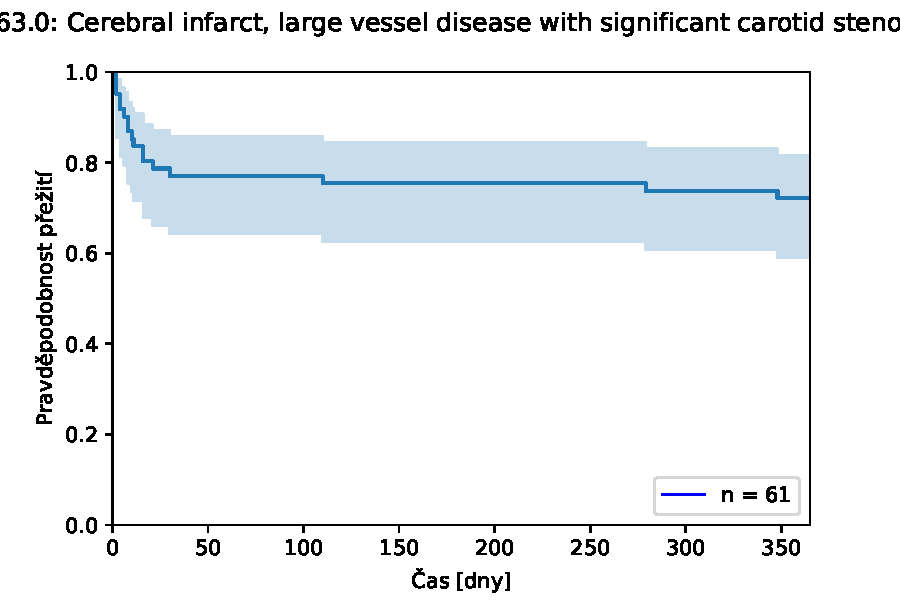
\includegraphics[width=65mm]{img/image_8.pdf}   & 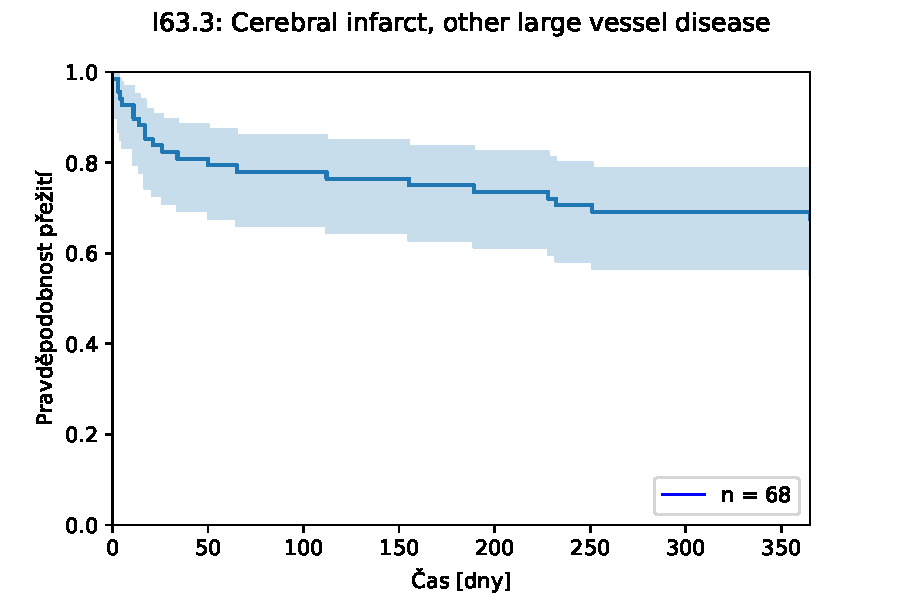
\includegraphics[width=65mm]{img/image_9.pdf}     \\    
        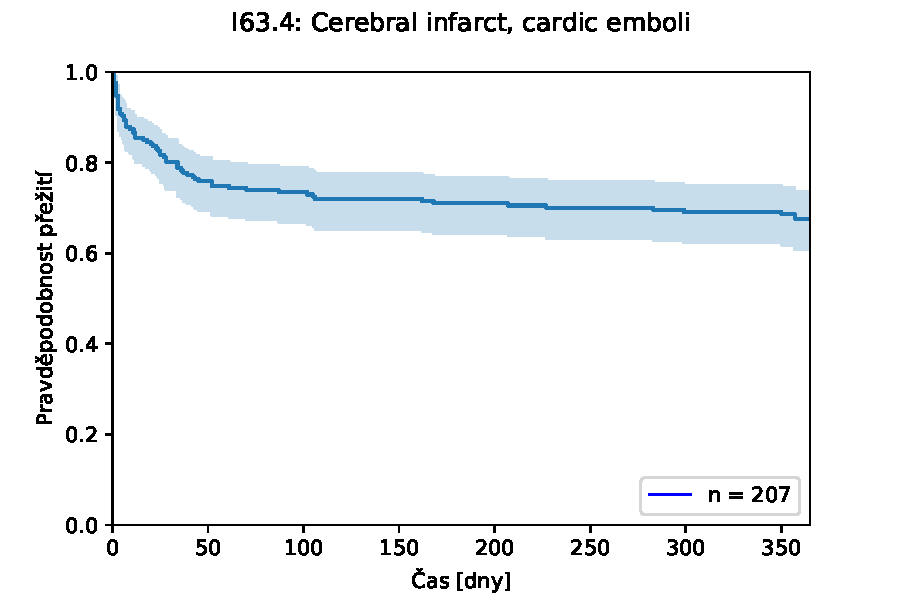
\includegraphics[width=65mm]{img/image_10.pdf}  & 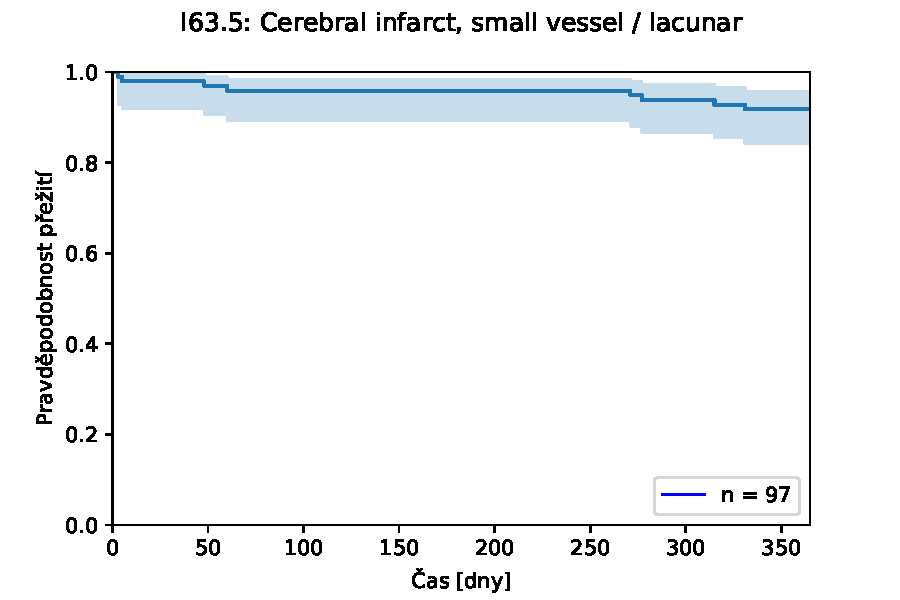
\includegraphics[width=65mm]{img/image_11.pdf}    \\
        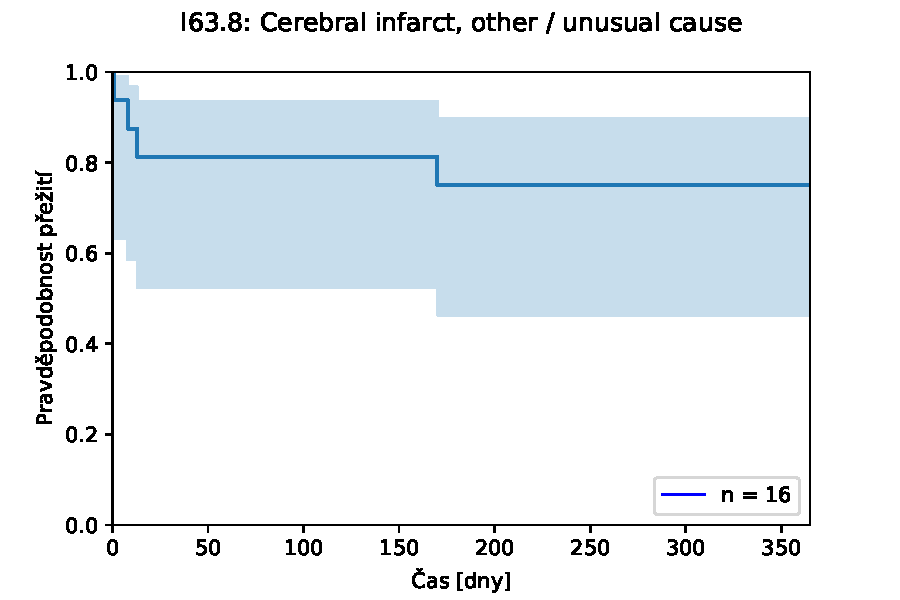
\includegraphics[width=65mm]{img/image_12.pdf}  & 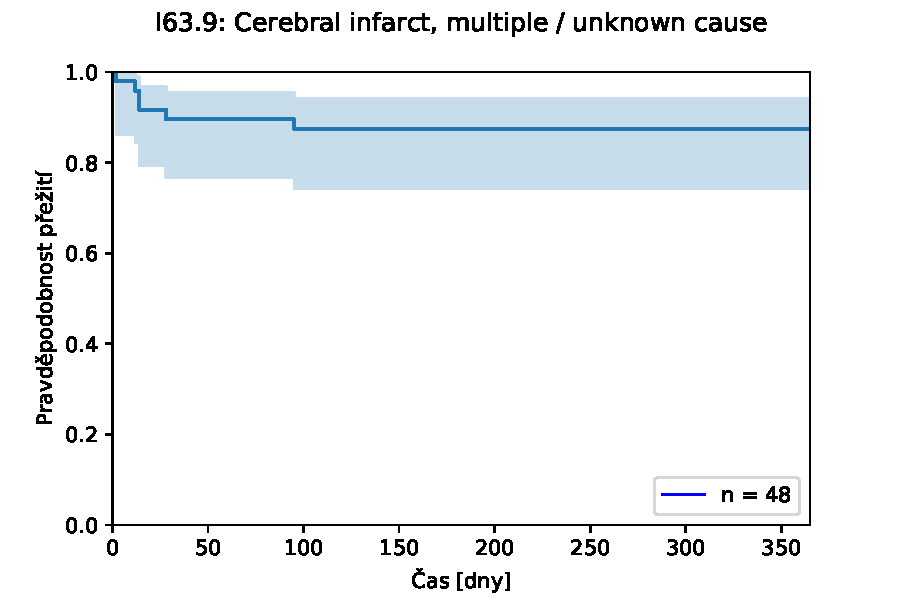
\includegraphics[width=65mm]{img/image_13.pdf}    \\
    
    \end{tabular}
    \centering
    \caption{Kaplan–Meierovy křivky přežití pro jednotlivé diagnózy}
\end{figure}
\FloatBarrier

\section{Závěr}

Úloha byla zajímavá především tím, že dala nahlédnout do problematiky metod analýzy přežití.
Kaplan–Meierova metoda je velice užitečnou technikou, která se dá na jednoduchých příkladech snadno spočítat i v ruce a může být případně využita i při výuce.
